\def\cG{\mathcal{G}}
\def\rr{\mathbb{R}}

\section{\lowrank: Gradient Low-Rank Projection}
\subsection{Background}


\textbf{Regular full-rank training.} At time step $t$, $G_t = -\nabla_W \phi_t(W_t) \in \rr^{m \times n}$ is the backpropagated (negative) gradient matrix. Then the regular pre-training weight update can be written down as follows ($\eta$ is the learning rate):
\begin{equation}
    W_T = W_0 + \eta \sum_{t=0}^{T-1} \tilde G_{t} = W_0 + \eta\sum_{t=0}^{T-1} \rho_t(G_t)
\end{equation}
where $\tilde G_t$ is the final processed gradient to be added to the weight matrix and $\rho_t$ is an entry-wise stateful gradient regularizer (e.g., Adam). The state of $\rho_t$ can be memory-intensive. For example, for Adam, we need $M,V \in \rr^{m\times n}$ to regularize the gradient $G_t$ into $\tilde G_{t}$:
\begin{eqnarray}
    M_t &=& \beta_1 M_{t-1} + (1-\beta_1) G_t \\  
    V_t &=& \beta_2 V_{t-1} + (1-\beta_2) G^2_t  \\
    \tilde G_t &=& M_t / \sqrt{V_t + \epsilon}
\end{eqnarray}
Here $G_t^2$ and $M_t / \sqrt{V_t + \epsilon}$ means element-wise multiplication and division. $\eta$ is the learning rate. Together with $W\in \rr^{m\times n}$, this takes $3mn$ memory. 

\textbf{Low-rank updates.} For a linear layer $W \in \mathbb{R}^{m \times n}$, LoRA and its variants utilize the low-rank structure of the update matrix by introducing a low-rank adaptor $AB$:
\begin{equation}
    W_T = W_0 + B_{T}A_{T},
\end{equation}
where $B \in \mathbb{R}^{m \times r}$ and $A \in \mathbb{R}^{r \times n}$, and $r \ll \min(m, n)$. $A$ and $B$ are the learnable low-rank adaptors and $W_0$ is a fixed weight matrix (e.g., pre-trained weight).

\subsection{Low-Rank Property of Weight Gradient}
While low-rank updates are proposed to reduce memory usage, it remains an open question whether the weight matrix should be parameterized as low-rank. In many situations, this may not be true. For example, in linear regression $\vy = W\vx$, if the optimal $W^*$ is high-rank, then imposing a low-rank assumption on $W$ never leads to the optimal solution, regardless of what optimizers are used. 

\def\beig{\lambda}
\def\ceig{\nu}

\def\bmin{\underline{\beig}}
\def\cmin{\underline{\ceig}}

\def\cN{\mathcal{N}}

Surprisingly, while the weight matrices are not necessarily low-rank, the gradient indeed becomes low-rank during the training for certain gradient forms and associated network architectures. 

\textbf{Reversible networks.} Obviously, for a general loss function, its gradient can be arbitrary and is not necessarily low rank. Here we study the gradient structure for a general family of nonlinear networks known as ``reversible networks''~\cite{tian2020understanding}, which includes not only simple linear networks but also deep ReLU/polynomial networks:

\begin{definition}[Reversiblity~\cite{tian2020understanding}]
A network $\cN$ that maps input $\vx$ to output $\vy = \cN(\vx)$ is \emph{reversible}, if there exists $L(\vx; W)$ so that $\vy= L(\vx; W)\vx$, and the backpropagated gradient $\vg_\vx$ satisfies $\vg_\vx = L^\top(\vx; W) \vg_\vy$, where $\vg_\vy$ is the backpropagated gradient at the output $\vy$. Here $L(\vx;W)$ depends on the input $\vx$ and weight $W$ in the network $\cN$. 
\end{definition}

Please check Appendix~\ref{sec:reversibility} for its properties. For reversible networks, the gradient takes a specific form. 

\begin{restatable}[Gradient Form of reversible models]{theorem}{gradientreversible}
\label{thm:gradientreversible}
Consider a chained reversible neural network $\cN(\vx) := \cN_L(\cN_{L-1}(\ldots\cN_1(\vx)))$ and define $J_l := \mathrm{Jacobian}(\cN_L) \ldots \mathrm{Jacobian}(\cN_{l+1})$ and $\vf_l := \cN_l(\ldots \cN_1(\vx))$. Then the weight matrix $W_l$ at layer $l$ has gradient $G_l$ in the following form for batch size 1:  

\textbf{(a)} For $\ell_2$-objective $\phi := \frac12\|\vy - \vf_L\|_2^2$: 
\begin{equation}
    G_l = \left(J_l^\top \vy - J^\top_l J_l W_l \vf_{l-1}\right)\vf_{l-1}^\top \label{eq:reversible-grad}
\end{equation}

\textbf{(b)} Left $P^\perp_\vone := I - \frac{1}{K}\vone\vone^\top$ be the zero-mean PSD projection matrix. For $K$-way logsoftmax loss $\phi(\vy; \vf_L) := -\log \left( \frac{\exp(\vy^\top \vf_L)}{\vone^\top \exp(\vf_L)}\right)$ with small logits $\|P^\perp_\vone\vf_L\|_\infty \ll \sqrt{K}$: 
\begin{equation}
    G_l = \left(J_lP^\perp_\vone \vy - \gamma K^{-1}J_l^\top P^\perp_\vone J_l W_l \vf_{l-1}\right)\vf_{l-1}^\top
\end{equation}
where $\gamma \approx 1$ and $\vy$ is a data label with $\vy^\top \vone = 1$.
\end{restatable}

\def\dd{\mathrm{d}}
\def\gzeroproj{G_{t_0}^\parallel}
\def\cV{\mathcal{V}}

From the theoretical analysis above, we can see that for batch size $N$, the gradient $G$ has certain structures: $G = \frac{1}{N}\sum_{i=1}^N (A_i - B_i W C_i)$ for input-dependent matrix $A_i$, Positive Semi-definite (PSD) matrices $B_i$ and $C_i$. In the following, we prove that such a gradient will become low-rank during training in certain conditions:

\def\sr{\mathrm{sr}}

\begin{restatable}[Gradient becomes low-rank during training]{lemma}{gradientlowrank}
\label{lemma:gradientlowrank}
    Suppose the gradient follows the parametric form: 
    \begin{eqnarray}
          G_t=\frac{1}{N}\sum_{i=1}^N (A_i-B_i W_t C_i)\label{eq:constantgradientcoeff}
    \end{eqnarray} 
    with constant $A_i$, PSD matrices $B_i$ and $C_i$ after $t \ge t_0$. We study vanilla SGD weight update: $W_t=W_{t-1}+\eta G_{t-1}$. Let $S := \frac{1}{N}\sum_{i=1}^N C_i \otimes B_i$ and $\lambda_1 < \lambda_2$ its two smallest distinct eigenvalues. Then the stable rank $\sr(G_t)$ satisfies:
    \begin{equation}
        \sr(G_t) \le \sr(\gzeroproj)\!+\!\left(\frac{1\!-\!\eta \lambda_2}{1\!-\!\eta \lambda_1}\right)^{2(t-t_0)} \frac{\|G_0\!-\!\gzeroproj\|_F^2}{\|\gzeroproj\|_2^2} \label{eq:stable-rank-decay}
    \end{equation}
    where $\gzeroproj$ is the projection of $G_{t_0}$ onto the minimal eigenspace $\cV_1$ of $S$ corresponding to $\lambda_1$.
\end{restatable}
In practice, the constant assumption can approximately hold for some time, in which the second term in Eq.~\ref{eq:stable-rank-decay} goes to zero exponentially and the stable rank of $G_t$ goes down, yielding low-rank gradient $G_t$. The final stable rank is determined by $\sr(\gzeroproj)$, which is estimated to be low-rank by the following: 
\begin{restatable}[Low-rank $G_t$]{corollary}{lowrankmid}
\label{co:low-rank-mid}
If the gradient takes the parametric form $G_t = \frac{1}{N}\sum_{i=1}^N (\va_i - B_i W_t \vf_i)\vf_i^\top$ with all $B_i$ full-rank, and $N' := \rank(\{\vf_i\}) < n$, then $\sr(\gzeroproj) \le n - N'$ and thus $\sr(G_t) \le n/2$ for large $t$. 
\end{restatable}
\textbf{Remarks.} The gradient form is justified by  Theorem~\ref{thm:gradientreversible}. Intuitively, when $N'$ is small, $G_t$ is a summation of $N'$ rank-1 update and is naturally low rank; on the other hand, when $N'$ becomes larger and closer to $n$, then the training dynamics has smaller null space $\cV_1$, which also makes $G_t$ low-rank. The full-rank assumption of $\{B_i\}$ is reasonable, e.g., in LLMs, the output dimensions of the networks (i.e., the vocabulary size) is often huge compared to matrix dimensions. 

In general if the batch size $N$ is large, then it becomes a bit tricky to characterize the minimal eigenspace $\cV_1$ of $S$. On the other hand, if $\cV_1$ has nice structure, then $\sr(G_t)$ can be bounded even further: 
\begin{restatable}[Low-rank $G_t$ with special structure of $\cV_1$]{corollary}{lowrankhigh}
If $\cV_1(S)$ is 1-dimensional with decomposable eigenvector $\vv = \vy \otimes \vz$, then $\sr(\gzeroproj) = 1$ and thus $G_t$ becomes rank-1.
\end{restatable}

One rare failure case of Lemma~\ref{lemma:gradientlowrank} is when $\gzeroproj$ is precisely zero, in which $\sr(\gzeroproj)$ becomes undefined. This happens to be true if $t_0 = 0$, i.e., $A_i$, $B_i$ and $C_i$ are constant throughout the entire training process. Fortunately, for practical training, this does not happen. 

\def\vdelta{\boldsymbol{\Delta}}

\textbf{Transformers.} For Transformers, we can also separately prove that the weight gradient of the lower layer (i.e., \emph{project-up}) weight of feed forward network (FFN) becomes low rank over time, using the JoMA framework~\cite{tian2023joma}. Please check Appendix (Sec.~\ref{sec:transformer-low-rank}) for details.  




\subsection{Gradient Low-rank Projection (\lowrank{})}
Since the gradient $G$ may have a low-rank structure, if we can keep the gradient statistics of a small ``core'' of gradient $G$ in optimizer states, rather than $G$ itself, then the memory consumption can be reduced substantially. This leads to our proposed \lowrank{} strategy: 
\begin{definition}[Gradient Low-rank Projection (\textbf{\lowrank})]
Gradient low-rank projection (\textbf{\lowrank}) denotes the following gradient update rules ($\eta$ is the learning rate):
\begin{equation}
    \label{eq:represent_low_rank_updates}
    W_T = W_0 + \eta\sum_{t=0}^{T-1} \tilde G_{t}, \quad \tilde G_t = P_t \rho_t(P_t^\top G_t Q_t) Q^\top_t
\end{equation}
where $P_t \in \mathbb{R}^{m \times r}$ and $Q_t \in \mathbb{R}^{n\times r}$ are projection matrices. 
\end{definition}
Different from LoRA, \lowrank{} \textit{explicitly utilizes the low-rank updates} instead of introducing additional low-rank adaptors and hence does not alter the training dynamics. 

In the following, we show that \lowrank{} converges under a similar (but more general) form of gradient update rule (Eqn.~\ref{eq:constantgradientcoeff}). This form corresponds to Eqn.~\ref{eq:reversible-grad} but with a larger batch size.  

\def\ee{\mathbb{E}}
\def\cW{\mathcal{W}}
\def\cN{\mathcal{N}}




\begin{definition}[$L$-continuity]
A function $\vh(W)$ has (Lipschitz) $L$-continuity, if for any $W_1$ and $W_2$, $\|\vh(W_1) - \vh(W_2)\|_F \le L\|W_1-W_2\|_F$. 
\end{definition}

\begin{restatable}[Convergence of \lowrank with fixed projections]{theorem}{convgpg}
    \label{thm:convgpg}
    Suppose the gradient has the form of Eqn.~\ref{eq:constantgradientcoeff} and $A_i$, $B_i$ and $C_i$ have $L_A$, $L_B$ and $L_C$ continuity with respect to $W$ and $\|W_t\|\le D$. Let $R_t := P_t^\top G_t Q_t$, $\hat B_{it} := P_t^\top B_{i}(W_t) P_t$, $\hat C_{it} := Q_t^\top C_i(W_t) Q_t$ and $\kappa_t := \frac1N \sum_i \lambda_{\min}(\hat B_{it}) \lambda_{\min}(\hat C_{it})$. If we choose constant $P_t = P$ and $Q_t=Q$, then \lowrank{} with $\rho_t \equiv 1$ satisfies:
    \begin{equation}
        \|R_t\|_F \le \left[1\!-\!\eta(\kappa_{t-1}\!-\!L_A\!-\!L_B L_C D^2)\right]\|R_{t-1}\|_F \label{eq:converge-rt}
    \end{equation}
    As a result, if $\min_t \kappa_t > L_A + L_B L_C D^2$, $R_t \rightarrow 0$ and thus \lowrank{} converges with fixed $P_t$ and $Q_t$.
\end{restatable}
\textbf{Setting $P$ and $Q$}. The theorem tells that $P$ and $Q$ should project into the subspaces corresponding to the first few largest eigenvectors of $\hat B_{it}$ and $\hat C_{it}$ for faster convergence (large $\kappa_t$). While all eigenvalues of the positive semidefinite (PSD) matrix $B$ and $C$ are non-negative, some of them can be very small and hinder convergence (i.e., it takes a long time for $G_t$ to become $0$). With the projection $P$ and $Q$, $P^\top B_{it} P$ and $Q^\top C_{it} Q$ only contain the largest eigen subspaces of $B$ and $C$, improving the convergence of $R_t$ and at the same time, reduces the memory usage. 

While it is tricky to obtain the eigenstructure of $\hat B_{it}$ and $\hat C_{it}$ (they are parts of Jacobian), one way is to instead use the spectrum of $G_t$ via Singular Value Decomposition (SVD): 
\begin{align}
    \label{eq:svd_p_q}
    G_t &= U S V^{\top} \approx \sum_{i=1}^{r} s_{i} u_{i} v_{i}^{\top} \\
    P_t &= [u_1, u_2, ..., u_r], 
    \quad
    Q_t = [v_1, v_2, ..., v_r]
\end{align}


\textbf{Difference between \lowrank{} and LoRA.}
While both \lowrank{} and LoRA have ``low-rank'' in their names, they follow very different training trajectories. For example, when $r = \min(m, n)$, \lowrank{} with $\rho_t \equiv 1$ follows the exact training trajectory of the original model, as $\tilde G_t = P_t P_t^{\top} G_t Q_t Q_t^\top = G_t$. On the other hand, when $BA$ reaches full rank (i.e., $B \in \mathbb{R}^{m \times m}$ and $A \in \mathbb{R}^{m \times n}$), optimizing $B$ and $A$ simultaneously follows a very different training trajectory compared to the original model.

\section{\lowrank{} for Memory-Efficient Training}
For a complex optimization problem such as LLM pre-training, it may be difficult to capture the entire gradient trajectory with a single low-rank subspace. One reason is that the principal subspaces of $B_t$ and $C_t$ (and thus $G_t$) may change over time. In fact, if we keep the same projection $P$ and $Q$, then the learned weights will only grow along these subspaces, which is not longer full-parameter training. Fortunately, for this, \lowrank{} can switch subspaces during training and learn full-rank weights without increasing the memory footprint.  


\subsection{Composition of Low-Rank Subspaces}
\label{sec:composition-subspace}
\begin{figure}
    \centering
    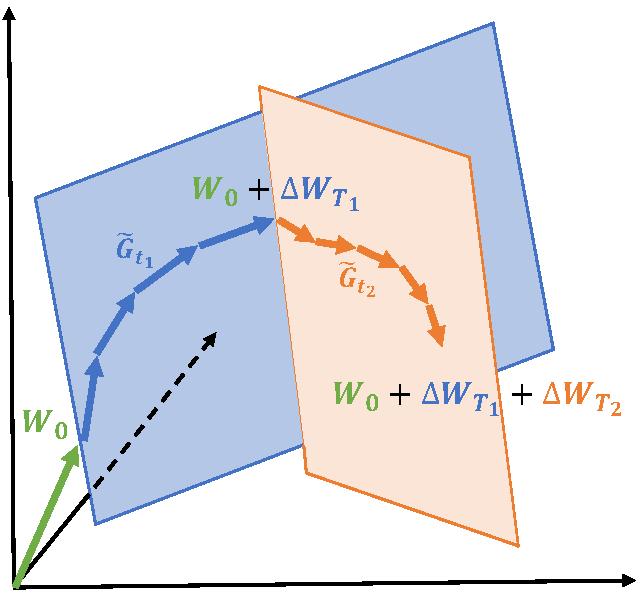
\includegraphics[width=0.58\linewidth]{figures/files/subspace_learning.pdf}
    \caption{\small{ Learning through low-rank subspaces $\Delta W_{T_1}$ and $\Delta W_{T_2}$ using \lowrank{}. For $t_1 \in [0, T_1 - 1]$, $W$ are updated by projected gradients $\tilde G_{t_1}$ in a subspace determined by fixed $P_{t_1}$ and $Q_{t_1}$. After $T_1$ steps, the subspace is changed by recomputing $P_{t_2}$ and $Q_{t_2}$ for $t_2 \in [T_1, T_2 - 1]$, and the process repeats until convergence.}}
    \label{fig:subspace_learning}
\vspace{-3mm}
\end{figure}

We allow \lowrank{} to switch across low-rank subspaces:
\begin{equation}
    \label{eq:represent_low_rank_updates_multiple}
    W_t = W_0 + \Delta W_{T_1} + \Delta W_{T_2} + \ldots + \Delta W_{T_n},
\end{equation}
where $t \in \left[\sum_{i=1}^{n-1} T_i, \sum_{i=1}^{n} T_i\right]$ and $\Delta W_{T_i} = \eta\sum_{t=0}^{T_i-1} \tilde{G_t}$ is the summation of all $T_i$ updates within the $i$-th subspace.
When switching to $i$-th subspace at step $t=T_i$, we re-initialize the projector $P_t$ and $Q_t$ by performing SVD on the current gradient $G_t$ by Equation \ref{eq:svd_p_q}.
We illustrate how the trajectory of $\tilde{G_t}$ traverses through multiple low-rank subspaces in Fig.~\ref{fig:subspace_learning}.
In the experiment section, we show that allowing multiple low-rank subspaces is the key to achieving the successful pre-training of LLMs.

Following the above procedure, the switching frequency $T$ becomes a hyperparameter. The ablation study (Fig.~\ref{fig:ablation}) shows a sweet spot exists. A very frequent subspace change increases the overhead (since new $P_t$ and $Q_t$ need to be computed) and breaks the condition of constant projection in Theorem~\ref{thm:convgpg}. In practice, it may also impact the fidelity of the optimizer states, which accumulate over multiple training steps. On the other hand, a less frequent change may make the algorithm stuck into a region that is no longer important to optimize (convergence proof in Theorem~\ref{thm:convgpg} only means good progress in the designated subspace, but does not mean good overall performance). While optimal $T$ depends on the total training iterations and task complexity, we find that a value between $T=50$ to $T=1000$ makes no much difference. Thus, the total computational overhead induced by SVD is negligible ($< 10\%$) compared to other memory-efficient training techniques such as memory offloading \citep{rajbhandariZeROMemoryOptimizations2020}.

\subsection{Memory-Efficient Optimization}

\newlength\myindent
\setlength\myindent{2em}
\newcommand\bindent{%
  \begingroup
  \setlength{\itemindent}{\myindent}
  \addtolength{\algorithmicindent}{\myindent}
}
\newcommand\eindent{\endgroup}



\begin{algorithm}[tb]
   \caption{Adam with \lowrank}
   \label{alg:low_rank_adam}
 \begin{algorithmic}
   \STATE {\bfseries Input:} A layer weight matrix $W \in \mathbb{R}^{m \times n}$ with $m \leq n$. Step size $\eta$, scale factor $\alpha$, decay rates $\beta_1, \beta_2$, rank $r$, subspace change frequency $T$.
   \STATE Initialize first-order moment $M_0 \in \mathbb{R}^{n \times r} \gets 0$
   \STATE Initialize second-order moment $V_0 \in \mathbb{R}^{n \times r} \gets 0$
   \STATE Initialize step $t \gets 0$
   \REPEAT
   \STATE $G_t \in \mathbb{R}^{m \times n} \gets - \nabla_W \phi_t(W_t)$ 
   \IF{$t \bmod T = 0$}
   \STATE $U, S, V \gets \text{SVD}(G_t)$
   \STATE $P_t \gets U[:, :r]$ \hfill \COMMENT{Initialize left projector as $m \leq n$}
   \ELSE
   \STATE $P_t \gets P_{t-1}$ \hfill \COMMENT{Reuse the previous projector}
   \ENDIF
   \STATE $R_t \gets P_{t}^{\top} G_t$ \hfill \COMMENT{Project gradient into compact space}
   \\\hrulefill
   \STATE {\bfseries $\update(R_t)$ by Adam}
   \bindent
   \hspace{\algorithmicindent} \STATE $M_t \gets \beta_1 \cdot M_{t-1} + (1 - \beta_1) \cdot R_t$ 
   \hspace{\algorithmicindent} \STATE $V_t \gets \beta_2 \cdot V_{t-1} + (1 - \beta_2) \cdot R_t^2$ 
   \hspace{\algorithmicindent} \STATE $M_t \gets M_t / (1 - \beta_1^t)$
   \hspace{\algorithmicindent} \STATE $V_t \gets V_t / (1 - \beta_2^t)$ 
   \hspace{\algorithmicindent} \STATE $N_t \gets M_t / (\sqrt{V_t} + \epsilon)$
   \eindent
   \\\hrulefill
   \STATE $\tilde G_t \gets \alpha \cdot P N_t$ \hfill \COMMENT{Project back to original space}
   \STATE $W_t \gets W_{t-1} + \eta \cdot \tilde G_t$
   \STATE $t \gets t + 1$
   \UNTIL{convergence criteria met}
   \RETURN $W_t$
 \end{algorithmic}
\end{algorithm}


\textbf{Reducing memory footprint of gradient statistics.} \lowrank{} significantly reduces the memory cost of optimizer that heavily rely on component-wise gradient statistics, such as Adam \citep{kingmaAdamMethodStochastic2014}. 
When $\rho_t \equiv \mathrm{Adam}$, by projecting $G_t$ into its low-rank form $R_t$, Adam's gradient regularizer $\rho_t(R_t)$ only needs to track low-rank gradient statistics.
where $M_t$ and $V_t$ are the first-order and second-order momentum, respectively. 
\lowrank{} computes the low-rank normalized gradient $N_t$ as follows:
\begin{equation}
    \label{eq:low_rank_normalized_gradient}
    N_t = \rho_t(R_t) = M_t / (\sqrt{V_t} + \epsilon).
\end{equation}
\lowrank{} can also apply to other optimizers (e.g., Adafactor) that have similar update rules and require a large amount of memory to store gradient statistics. 
\paragraph{Reducing memory usage of projection matrices.} To achieve the best memory-performance trade-off, we only use one project matrix $P$ or $Q$, projecting the gradient $G$ into $P^\top G$ if $m \leq n$ and $G Q$ otherwise. We present the algorithm applying \lowrank{} to Adam in Algorithm~\ref{alg:low_rank_adam}. 

With this setting, \lowrank{} requires less memory than LoRA during training.
As \lowrank{} can always merge $\Delta W_t$ to $W_0$ during weight updates, it does not need to store a separate low-rank factorization $BA$.
In total, \lowrank{} requires $(mn + mr + 2nr)$ memory, while LoRA requires $(mn + 3mr + 3nr)$ memory.
A comparison between \lowrank{} and LoRA is shown in Table~\ref{tab:lora_compare}.

As Theorem \ref{thm:convgpg} does not require the projection matrix to be carefully calibrated, we can further reduce the memory cost of projection matrices by quantization and efficient parameterization, which we leave for future work.

\subsection{Combining with Existing Techniques}

\lowrank{} is compatible with existing memory-efficient optimization techniques.
In our work, we mainly consider applying \lowrank{} with 8-bit optimizers and per-layer weight updates.

\paragraph{8-bit optimizers.}
\citet{dettmers8bitOptimizersBlockwise2021} proposed 8-bit Adam optimizer that maintains 32-bit optimizer performance at a fraction of the memory footprint.
We apply \lowrank{} directly to the existing implementation of 8-bit Adam.

\paragraph{Per-layer weight updates.}
In practice, the optimizer typically performs a single weight update for all layers after backpropagation. This is done by storing the entire weight gradients in memory. 
To further reduce the memory footprint during training, we adopt per-layer weight updates to \lowrank, which performs the weight updates during backpropagation. This is the same technique proposed in recent works to reduce memory requirement \citep{lvAdaLomoLowmemoryOptimization2023,lvFullParameterFinetuning2023}.



\subsection{Hyperparameters of \lowrank{}}
\label{sec:lowrank-hyperparams}


In addition to Adam's original hyperparameters, \lowrank{} only introduces very few additional hyperparameters: the rank $r$ which is also present in LoRA, the subspace change frequency $T$ (see Sec.~\ref{sec:composition-subspace}), and the scale factor $\alpha$. 

Scale factor $\alpha$ controls the strength of the low-rank update, which is similar to the scale factor $\alpha/r$ appended to the low-rank adaptor in \citet{huLoRALowRankAdaptation2021}.
We note that the $\alpha$ does not depend on the rank $r$ in our case. 
This is because, when $r$ is small during pre-training, $\alpha/r$ significantly affects the convergence rate, unlike fine-tuning.




\begin{table}[t]
    \caption{\small{Comparison between \lowrank{} and LoRA. Assume $W \in \mathbb{R}^{m \times n}$ ($m \leq n$), rank $r$.}}
    
    \label{tab:lora_compare}
    \begin{center}
    \begin{small}
    \begin{tabular}{lcc}
    \toprule
               & \lowrank{} & LoRA \\
    \midrule
    Weights          & $mn$   & $mn+mr+nr$ \\
    Optim States           & $mr + 2nr$   & $2mr + 2nr$  \\
    \midrule
    Multi-Subspace   & \cmark   & \xmark \\
    Pre-Training   & \cmark   & \xmark \\
    Fine-Tuning   & \cmark   & \cmark \\
    \bottomrule
    \end{tabular}
    \end{small}
    \end{center}
\vspace{-6mm}
\end{table}


\section{Methods}

Natural gradient methods are optimization algorithms that adjust parameter updates according to the geometry of the parameter space, leading to faster convergence compared to standard gradient descent. They precondition the gradient using the inverse of the Fisher Information Matrix (FIM). However, computing and storing the full FIM and its inverse is computationally infeasible for large-scale models due to their high dimensionality.

To address this challenge, we propose an \textbf{online natural gradient algorithm} that operates in a low-rank subspace of the gradient space. By projecting gradients onto this subspace and approximating the FIM within it, we can efficiently compute natural gradient updates without explicit layer-wise information.

\subsection{Algorithm Description}

The algorithm consists of the following key steps:

\begin{enumerate}
    \item \textbf{Low-Rank Gradient Projection}
    \item \textbf{Gradient History Buffer Maintenance}
    \item \textbf{FIM Approximation Using Gradient History}
    \item \textbf{Natural Gradient Computation via Woodbury Identity}
    \item \textbf{Efficient Computation Using Cholesky Decomposition}
\end{enumerate}

We will explain each step in detail.

\subsubsection{Step 1: Low-Rank Gradient Projection}

Given a full-rank gradient tensor $\boldsymbol{g} \in \mathbb{R}^{n_1 \times n_2 \times \cdots \times n_d}$, we project it onto a low-rank subspace using Tucker decomposition. The Tucker decomposition approximates $\boldsymbol{g}$ as:

\[
\boldsymbol{g} \approx \mathcal{G} = \mathcal{C} \times_1 \mathbf{U}^{(1)} \times_2 \mathbf{U}^{(2)} \times_3 \cdots \times_d \mathbf{U}^{(d)},
\]

where:

\begin{itemize}
    \item $\mathcal{C} \in \mathbb{R}^{r_1 \times r_2 \times \cdots \times r_d}$ is the core tensor.
    \item $\mathbf{U}^{(i)} \in \mathbb{R}^{n_i \times r_i}$ are the factor matrices (orthogonal matrices).
    \item $\times_i$ denotes the mode-$i$ tensor-matrix product.
    \item $r_i$ is the rank along mode $i$, with $r_i \ll n_i$.
\end{itemize}

The low-rank representation (transformed gradient) is obtained by:

\[
\boldsymbol{g}_{\text{low}} = \text{Transform}(\boldsymbol{g}) = \boldsymbol{g} \times_1 (\mathbf{U}^{(1)})^\top \times_2 (\mathbf{U}^{(2)})^\top \times_3 \cdots \times_d (\mathbf{U}^{(d)})^\top.
\]

\subsubsection{Step 2: Gradient History Buffer Maintenance}

We maintain a buffer of the recent $s$ low-rank gradient vectors to capture local curvature information. Let $\boldsymbol{g}_t$ be the transformed low-rank gradient at iteration $t$, flattened into a vector:

\[
\boldsymbol{g}_t \in \mathbb{R}^{k}, \quad \text{where } k = r_1 r_2 \cdots r_d.
\]

We store the recent $s$ gradients in the matrix $\mathbf{G}$:

\[
\mathbf{G} = [\boldsymbol{g}_{t - s + 1}, \boldsymbol{g}_{t - s + 2}, \dots, \boldsymbol{g}_t] \in \mathbb{R}^{k \times s}.
\]

\subsubsection{Step 3: Approximating the Fisher Information Matrix}

We approximate the FIM within the low-rank subspace using the outer products of the stored gradients:

\[
\mathbf{F} = \lambda \mathbf{I}_k + \mathbf{G} \mathbf{G}^\top,
\]

where:

\begin{itemize}
    \item $\lambda > 0$ is a damping term to ensure numerical stability.
    \item $\mathbf{I}_k$ is the $k \times k$ identity matrix.
\end{itemize}

\subsubsection{Step 4: Computing the Natural Gradient via Woodbury Identity}

Directly computing $\mathbf{F}^{-1}$ is computationally expensive for large $k$. Instead, we use the \textbf{Woodbury identity} to efficiently compute $\mathbf{F}^{-1} \boldsymbol{g}_t$:

\[
\mathbf{F}^{-1} \boldsymbol{g}_t = \frac{1}{\lambda} \left( \boldsymbol{g}_t - \mathbf{G} \left( \lambda \mathbf{I}_s + \mathbf{G}^\top \mathbf{G} \right)^{-1} \mathbf{G}^\top \boldsymbol{g}_t \right).
\]

Let us define:

\begin{itemize}
    \item $\mathbf{S} = \lambda \mathbf{I}_s + \mathbf{G}^\top \mathbf{G} \in \mathbb{R}^{s \times s}$.
    \item $\boldsymbol{y} = \mathbf{G}^\top \boldsymbol{g}_t \in \mathbb{R}^s$.
\end{itemize}

Then, we compute:

\begin{enumerate}
    \item $\mathbf{S} = \lambda \mathbf{I}_s + \mathbf{G}^\top \mathbf{G}$.
    \item Solve $\mathbf{S} \boldsymbol{z} = \boldsymbol{y}$ for $\boldsymbol{z}$.
    \item Compute $\mathbf{F}^{-1} \boldsymbol{g}_t = \dfrac{1}{\lambda} \left( \boldsymbol{g}_t - \mathbf{G} \boldsymbol{z} \right)$.
\end{enumerate}

\subsubsection{Step 5: Efficient Computation Using Cholesky Decomposition}

To efficiently solve the linear system $\mathbf{S} \boldsymbol{z} = \boldsymbol{y}$, we use \textbf{Cholesky decomposition}:

\begin{enumerate}
    \item Compute the Cholesky factorization of $\mathbf{S}$:

    \[
    \mathbf{S} = \mathbf{L} \mathbf{L}^\top,
    \]

    where $\mathbf{L}$ is a lower triangular matrix.

    \item Solve for $\boldsymbol{u}$ in the forward substitution:

    \[
    \mathbf{L} \boldsymbol{u} = \boldsymbol{y}.
    \]

    \item Solve for $\boldsymbol{z}$ in the backward substitution:

    \[
    \mathbf{L}^\top \boldsymbol{z} = \boldsymbol{u}.
    \]
\end{enumerate}

\subsection{Algorithm Summary}

At each iteration $t$, the algorithm proceeds as follows:

\begin{enumerate}
    \item \textbf{Project the Full-Rank Gradient}:

    \begin{itemize}
        \item Obtain the low-rank transformed gradient $\boldsymbol{g}_t$ using the current factors $\{\mathbf{U}^{(i)}\}$.
    \end{itemize}

    \item \textbf{Update Gradient History}:

    \begin{itemize}
        \item If the history buffer is full, remove the oldest gradient.
        \item Add $\boldsymbol{g}_t$ to the history buffer $\mathbf{G}$.
    \end{itemize}

    \item \textbf{Compute Intermediate Quantities}:

    \begin{itemize}
        \item $\mathbf{S} = \lambda \mathbf{I}_s + \mathbf{G}^\top \mathbf{G}$.
        \item $\boldsymbol{y} = \mathbf{G}^\top \boldsymbol{g}_t$.
    \end{itemize}

    \item \textbf{Solve for $\boldsymbol{z}$}:

    \begin{itemize}
        \item Use Cholesky decomposition of $\mathbf{S}$ to solve $\mathbf{S} \boldsymbol{z} = \boldsymbol{y}$.
    \end{itemize}

    \item \textbf{Compute the Natural Gradient}:

    \begin{itemize}
        \item $\tilde{\boldsymbol{g}}_t = \dfrac{1}{\lambda} \left( \boldsymbol{g}_t - \mathbf{G} \boldsymbol{z} \right)$.
    \end{itemize}

    \item \textbf{Reshape and Project Back}:

    \begin{itemize}
        \item Reshape $\tilde{\boldsymbol{g}}_t$ back to the low-rank tensor shape.
        \item Optionally, project back to the full parameter space using the inverse transform.
    \end{itemize}
\end{enumerate}

\subsection{Mathematical Formulas}

\subsubsection{Low-Rank Projection}

The transformed low-rank gradient is obtained by:

\[
\boldsymbol{g}_{\text{low}} = \boldsymbol{g} \times_1 (\mathbf{U}^{(1)})^\top \times_2 (\mathbf{U}^{(2)})^\top \times_3 \cdots \times_d (\mathbf{U}^{(d)})^\top.
\]

\subsubsection{FIM Approximation}

We approximate the FIM as:

\[
\mathbf{F} = \lambda \mathbf{I}_k + \mathbf{G} \mathbf{G}^\top.
\]

\subsubsection{Natural Gradient Computation}

Compute the natural gradient using:

\[
\tilde{\boldsymbol{g}}_t = \mathbf{F}^{-1} \boldsymbol{g}_t = \dfrac{1}{\lambda} \left( \boldsymbol{g}_t - \mathbf{G} \boldsymbol{z} \right),
\]

where $\boldsymbol{z}$ solves:

\[
\left( \lambda \mathbf{I}_s + \mathbf{G}^\top \mathbf{G} \right) \boldsymbol{z} = \mathbf{G}^\top \boldsymbol{g}_t.
\]

\subsubsection{Efficient Solution via Cholesky Decomposition}

\begin{enumerate}
    \item Compute $\mathbf{L}$ such that:

    \[
    \lambda \mathbf{I}_s + \mathbf{G}^\top \mathbf{G} = \mathbf{L} \mathbf{L}^\top.
    \]

    \item Solve for $\boldsymbol{u}$:

    \[
    \mathbf{L} \boldsymbol{u} = \boldsymbol{y}.
    \]

    \item Solve for $\boldsymbol{z}$:

    \[
    \mathbf{L}^\top \boldsymbol{z} = \boldsymbol{u}.
    \]

    \item Compute the natural gradient:

    \[
    \tilde{\boldsymbol{g}}_t = \dfrac{1}{\lambda} \left( \boldsymbol{g}_t - \mathbf{G} \boldsymbol{z} \right).
    \]
\end{enumerate}

\subsection{Notes on Implementation}

\subsubsection{Avoiding Large Matrix Inversions}

By using the Woodbury identity and Cholesky decomposition, we avoid inverting large matrices of size $k \times k$, where $k$ can be very large.

\subsubsection{Computational Efficiency}

\begin{itemize}
    \item \textbf{Matrix-Vector Products}: Preferred over matrix-matrix multiplications for efficiency on GPUs.
    \item \textbf{GPU Computation}: All tensors are kept on the GPU to avoid data transfer overhead.
    \item \textbf{Efficient Linear Algebra}: Utilizing optimized GPU routines for operations like matrix multiplication and Cholesky decomposition.
\end{itemize}

\subsubsection{Memory Efficiency}

The history size $s$ is kept small (e.g., $s = 10$) to limit memory usage and computational cost.

\subsubsection{Numerical Stability}

The damping term $\lambda$ ensures that $\mathbf{S}$ is positive definite, allowing for stable Cholesky decomposition.

\subsection{Conclusion}

The proposed online natural gradient algorithm efficiently approximates the natural gradient in a low-rank subspace without requiring explicit layer-wise information. By maintaining a history of recent low-rank gradients and utilizing the Woodbury identity along with Cholesky decomposition, we can compute natural gradient updates efficiently on GPUs. This makes the method suitable for large-scale optimization problems where full natural gradient methods are computationally prohibitive.